\documentclass[14pt,a4paper]{extarticle}
\usepackage[T2A]{fontenc}
\usepackage[utf8]{inputenc}
\usepackage[english,russian]{babel}
\usepackage{lmodern}
\usepackage{geometry}
\usepackage{array}
\usepackage{tabularx}
\usepackage{longtable}
\usepackage{ltablex}
\usepackage{booktabs}
\usepackage{hyperref}
\usepackage{indentfirst}
\usepackage{microtype}
\usepackage{graphicx}
\usepackage{setspace}
\usepackage{listings}
\usepackage{graphicx}
\usepackage{caption}
\usepackage{float}
\usepackage{tocloft}
\usepackage{titlesec}
\usepackage{newtxtext,newtxmath}

\titleformat{\section}        % форматируем \section
  {\normalfont\bfseries}      % стиль: обычный + жирный
  {\thesection.}              % номер секции с точкой
  {2mm}                       % расстояние между номером и текстом
  {}                           % перед заголовком можно добавить что-то
\titlespacing*{\section}{1.5cm}{*3}{*1}  % {отступ слева}{отступ сверху}{отступ снизу}

\titleformat{\subsection}        % форматируем \section
  {\normalfont\bfseries}      % стиль: обычный + жирный
  {\thesubsection.}              % номер секции с точкой
  {2mm}                       % расстояние между номером и текстом
  {}                           % перед заголовком можно добавить что-то
\titlespacing*{\subsection}{1.5cm}{*3}{*1}  % {отступ слева}{отступ сверху}{отступ снизу}

\captionsetup{justification=centering}
\renewcommand{\ttdefault}{cmtt}
\keepXColumns
\setlength{\parindent}{3em}
\newgeometry{left=2.5cm,right=2.5cm,top=3cm,bottom=2.5cm}
\graphicspath{{../}{./}}

\renewcommand{\contentsname}{\hspace*{4em}{\smallСодержание}}
\setlength{\cftbeforesecskip}{0.5em}
\renewcommand{\cftsecleader}{\cftdotfill{\cftdotsep}}
\renewcommand{\cftsecaftersnum}{.\hspace{2mm}}

\title{Отчёт по "Управление ИТ-проектами"}
\author{Выполнил студент группы М-РИТ-25-1, Станиславчук Сергей}

\begin{document}

\setstretch{1.5}
\noindent
\begin{minipage}[t]{0.01\textwidth}
    \includegraphics{~/programmer/++Programmer/5_1/LSTU.jpg}
\end{minipage}%
\begin{minipage}[c]{1.1\linewidth}
    \centering
    {\small
    МИНИСТЕРСТВО НАУКИ И ВЫСШЕГО ОБРАЗОВАНИЯ РФ \\[1em]
    ФЕДЕРАЛЬНОЕ ГОСУДАРСТВЕННОЕ БЮДЖЕТНОЕ \\
    ОБРАЗОВАТЕЛЬНОЕ УЧРЕЖДЕНИЕ ВЫСШЕГО ОБРАЗОВАНИЯ \\
    «ЛИПЕЦКИЙ ГОСУДАРСТВЕННЫЙ ТЕХНИЧЕСКИЙ УНИВЕРСИТЕТ»
    }
\end{minipage}%

\vspace{3em}

\noindent
\hspace{1em}%
\begin{minipage}[t]{0.8\textwidth}
\textbf{Институт} \hspace{2em} компьютерных наук \\
\textbf{Кафедра} \hspace{2em} автоматизированных систем управления
\end{minipage}


\vspace{6em}

\begin{center}
\textbf{Лабораторная работа №1} \\
по дисциплине \\ <<Прикладные задачи искусственного интеллекта>>
\end{center}

\vspace{6em}

\noindent
\begin{tabular*}{\textwidth}{@{\extracolsep{\fill}} l c r }
    Студент М-РИТ-25-1 & \makebox[4cm]{\hrulefill} & Станиславчук С.М. \\[2em]
Руководитель & \\
Профессор & \makebox[4cm]{\hrulefill} & Седых И.А. \\
\end{tabular*}

\vfill
\begin{center}
    Липецк, 2026
\end{center}

\thispagestyle{empty}

\newpage
\tableofcontents
\newpage

\section{Задание}

Цель работы --- решить задачу классификации текста двумя способами: классическим
методом (TF-IDF и логистическая регрессия) и дообучением (fine-tuning) предобученного
трансформера DistilBERT, сравнить их по качеству и времени обучения, по кривым
обучения количественно оценить переобучение и провести один управляемый эксперимент,
заданный вариантом.

\textbf{Вариант 16.} Датасет \texttt{financial\_phrasebank} в разметке

\texttt{sentences\_allagree} (все аннотаторы согласны с меткой), задача ---
тональность финансовых новостей; число классов $K=3$ (\texttt{negative},
\texttt{neutral}, \texttt{positive}); \texttt{MAX\_LEN}~$=64$. Оригинальный датасет
загружается только скриптом, поэтому используется parquet-зеркало

\texttt{gtfintechlab/financial\_phrasebank\_sentences\_allagree}. Номер варианта и
зерно: \texttt{SEED}~$=1016$; число эпох и скорость обучения:
\texttt{EPOCHS}~$=5$, \texttt{LR}~$=2\cdot10^{-5}$.

Эксперимент шага 3.4 (качество разметки): основная модель обучается на данных, где
все аннотаторы согласны с меткой. Нужно взять из зеркала
\texttt{warwickai/financial\_phrasebank\_mirror} (\texttt{ds50}, согласие не менее
50\,\% аннотаторов) столько же примеров, сколько в обучающей части, исключив
предложения валидации и теста, обучить модель с теми же настройками и оценить на
той же тестовой части.

Все данные приведены к двум колонкам \texttt{text}/\texttt{label} и разбиты в
пропорции 70/15/15: обучающая часть 1584 примера, валидационная --- 340,
тестовая --- 340. Все сравнения выполняются на одной и той же тестовой части.

\section{Ход работы}

\subsection{Задание 1. Разведка данных и классический baseline}

Распределение классов в обучающей части приведено в таблице~\ref{tab:classes}.
Виден выраженный дисбаланс: нейтральных новостей почти в пять раз больше, чем
негативных, поэтому наряду с Accuracy используется Macro-F1.

\begin{table}[H]
    \centering
    \begin{tabular}{lrr}
        \toprule
        Класс & Число примеров & Доля \\
        \midrule
        negative & 204 & 12{,}88\,\% \\
        neutral  & 978 & 61{,}74\,\% \\
        positive & 402 & 25{,}38\,\% \\
        \midrule
        Итого    & 1584 & 100\,\% \\
        \bottomrule
    \end{tabular}
    \caption{Распределение классов в обучающей части}
    \label{tab:classes}
\end{table}

На рисунке~\ref{fig:eda} показаны распределение классов и гистограмма длин текстов
в токенах токенизатора DistilBERT.

\begin{figure}[H]
    \centering
    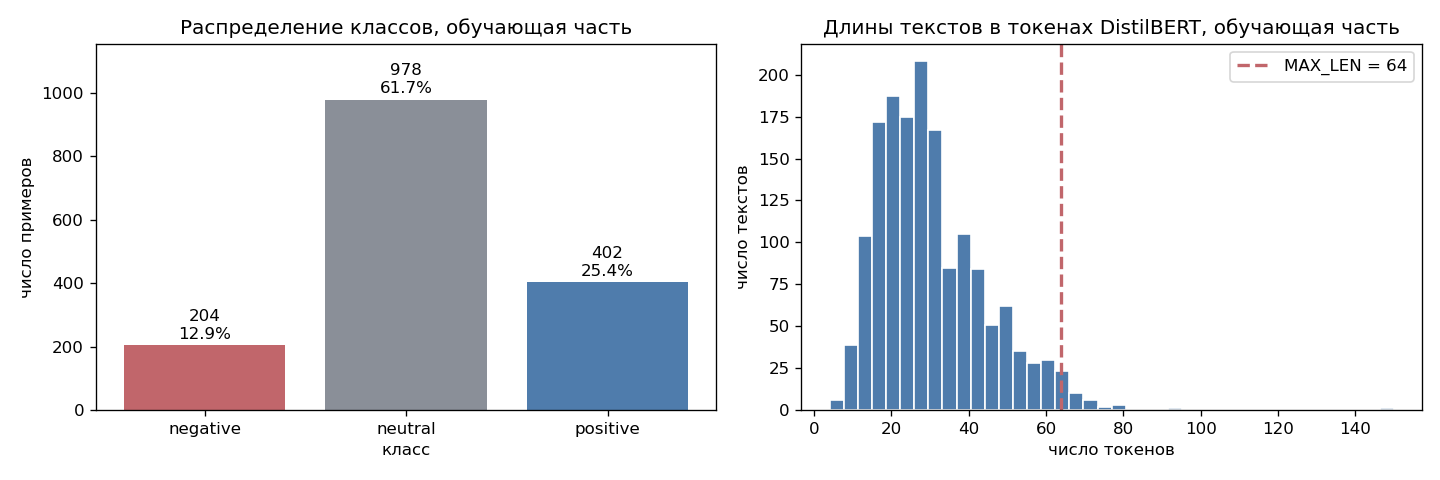
\includegraphics[width=\textwidth]{eda_plot.png}
    \refstepcounter{figure}
    \caption*{Рисунок \thefigure\ — Распределение классов (слева) и длины текстов в
    токенах DistilBERT (справа)}
    \label{fig:eda}
\end{figure}

Длины текстов: минимум 4, средняя 30.4, медиана 28, 90-й процентиль 50,
максимум 150 токенов. Доля текстов длиннее \texttt{MAX\_LEN}~$=64$ приведена в
таблице~\ref{tab:trunc}: в обучающей части обрезается 1.96\,\% текстов, в
валидационной --- 2.35\,\%, в тестовой --- 1.47\,\%. Потери информации из-за
усечения невелики, так как подавляющее большинство предложений короче 64 токенов.

\begin{table}[H]
    \centering
    \begin{tabular}{lrrr}
        \toprule
        Часть & Число текстов & Длиннее 64 & Доля \\
        \midrule
        обучающая    & 1584 & 31 & 1.96\,\% \\
        валидационная & 340 & 8  & 2.35\,\% \\
        тестовая      & 340 & 5  & 1.47\,\% \\
        \bottomrule
    \end{tabular}
    \caption{Доля текстов, обрезаемых при \texttt{MAX\_LEN}~$=64$}
    \label{tab:trunc}
\end{table}

Классический baseline: конвейер TF-IDF (\texttt{max\_features}~$=10000$, реально
получилось 4967 признаков) $\to$ логистическая регрессия
(\texttt{max\_iter}~$=1000$). Время обучения --- 0.2~с, Accuracy на тесте
0.8265, Macro-F1 0.7437. Отчёт по классам baseline приведён в
таблице~\ref{tab:base_report}.

\begin{table}[H]
    \centering
    \refstepcounter{table}
    \caption*{\raggedleft Таблица \thetable\ --- Отчет по классам baseline по тестовой части}
    \label{tab:base_report}
    \begin{tabular}{lrrrr}
        \toprule
        Класс & Precision & Recall & F1-score & Support \\
        \midrule
        negative & 0.8571 & 0.4706 & 0.6076 & 51 \\
        neutral  & 0.8279 & 0.9854 & 0.8998 & 205 \\
        positive & 0.8088 & 0.6548 & 0.7237 & 84 \\
        \midrule
        micro avg & 0.8265 & 0.8265 & 0.8265 & 340 \\
        macro avg & 0.8313 & 0.7036 & 0.7437 & 340 \\
        \bottomrule
    \end{tabular}
\end{table}

\noindent\textbf{Вывод по заданию 1.} Данные сильно несбалансированы (61{,}7\,\%
нейтральных против 12{,}9\,\% негативных), но усечению при \texttt{MAX\_LEN}~$=64$
подвергается менее 2{,}4\,\% текстов. TF-IDF + логистическая регрессия даёт
Accuracy 0{,}8265 и Macro-F1 0{,}7437, причём основной провал --- по редкому
классу \texttt{negative} (Recall 0{,}47): модель относит негативные новости к
нейтральным. Обучение практически мгновенное (0{,}2~с), поэтому baseline удобен
как точка отсчёта, но качество ограничено ``мешком слов'' без учёта контекста.

\subsection{Задание 2. Дообучение предобученного трансформера}

Дообучена модель \texttt{distilbert-base-uncased} с классификационной головой на
$K=3$. Вход обрезается до \texttt{MAX\_LEN}~$=64$; валидация и сохранение --- после
каждой эпохи, лучшая модель выбирается по \texttt{val Macro-F1}, включена ранняя
остановка с \texttt{patience}~$=2$. Динамика обучения по эпохам приведена в
таблице~\ref{tab:curves}, кривые --- на рисунке~\ref{fig:curves}.

\begin{table}[H]
    \centering
    \begin{tabular}{crrrr}
        \toprule
        Эпоха & Train loss & Val loss & Val Accuracy & Val Macro-F1 \\
        \midrule
        1 & 0{,}5764 & 0{,}2635 & 0{,}9294 & 0{,}8977 \\
        2 & 0{,}1478 & 0{,}1467 & 0{,}9559 & 0{,}9363 \\
        3 & 0{,}0597 & 0{,}1611 & 0{,}9588 & 0{,}9390 \\
        4 & 0{,}0375 & 0{,}1647 & 0{,}9588 & 0{,}9388 \\
        5 & 0{,}0257 & \textbf{0{,}1338} & \textbf{0{,}9618} & \textbf{0{,}9420} \\
        \bottomrule
    \end{tabular}
    \caption{Кривые обучения DistilBERT на валидационной части}
    \label{tab:curves}
\end{table}

\begin{figure}[H]
    \centering
    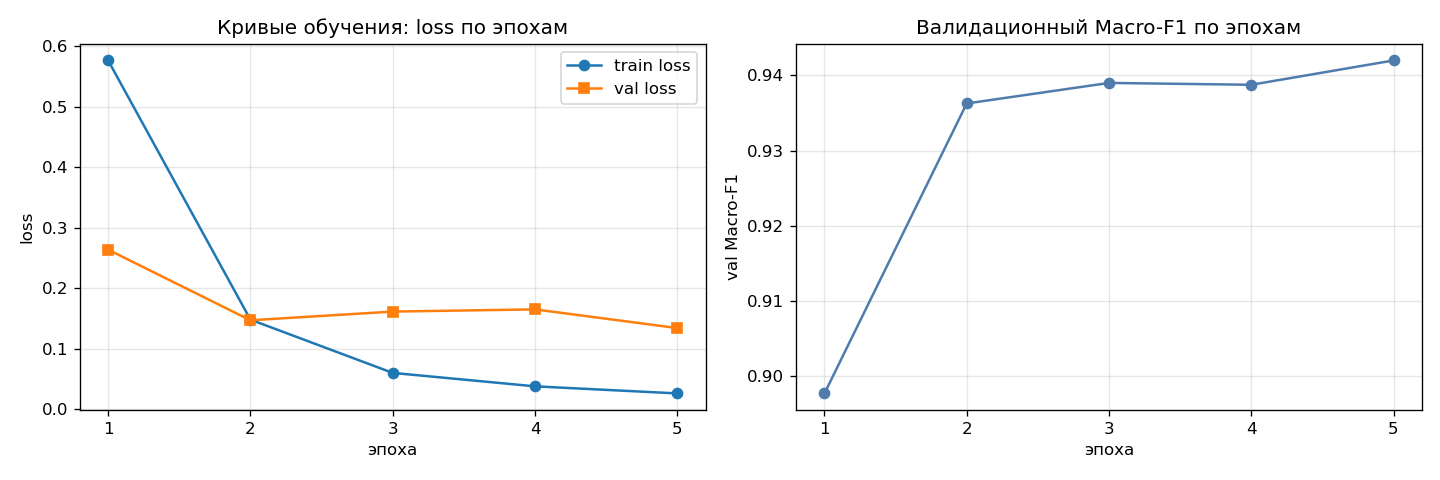
\includegraphics[width=\textwidth]{learning_curves.png}
    \caption{Кривые обучения: train loss и val loss (слева) и валидационный
    Macro-F1 (справа) по эпохам}
    \label{fig:curves}
\end{figure}

Время обучения основной модели --- 282{,}6~с (5 эпох, 495 шагов). Ранняя остановка
не сработала: выполнены все 5 эпох. На тестовой части получены Accuracy 0{,}9529,
Macro-F1 0{,}9321, test loss 0{,}1606. Сводное сравнение baseline и DistilBERT
приведено в таблице~\ref{tab:compare}.

\begin{table}[H]
    \centering
    \begin{tabular}{lrrr}
        \toprule
        Постановка & Accuracy & Macro-F1 & Время, с \\
        \midrule
        TF-IDF + LogReg (baseline) & 0{,}8265 & 0{,}7437 & 0{,}2 \\
        DistilBERT (дообучение)    & 0{,}9529 & 0{,}9321 & 282{,}6 \\
        \bottomrule
    \end{tabular}
    \caption{Сравнение baseline и DistilBERT на одной тестовой части}
    \label{tab:compare}
\end{table}

\noindent\textbf{Вывод по заданию 2.} Дообучение DistilBERT даёт Accuracy 0{,}9529
и Macro-F1 0{,}9321 против 0{,}8265 и 0{,}7437 у baseline: прирост Macro-F1
составляет почти 19 процентных пунктов, при этом модель обучалась всего 5 эпох. Плата
за качество --- время: 282{,}6~с против 0{,}2~с, то есть трансформер примерно в
1400 раз дороже по обучению при несопоставимо лучшем качестве. Кривые показывают,
что val loss снижается почти монотонно до последней эпохи, а ранняя остановка не
потребовалась.

\subsection{Задание 3. Анализ переобучения и ошибок}

\textbf{Шаг 3.1. Анализ переобучения.} По кривым из задания~2 минимум val loss и
максимум val Macro-F1 приходятся на одну и ту же (последнюю) эпоху~5:
val loss~$=0{,}1338$, val Macro-F1~$=0{,}9420$. Разрыв между валидационной и
обучающей потерями на последней эпохе составляет $0{,}1338 - 0{,}0257 = +0{,}1081$.
Ранняя остановка не сработала (выполнены 5 из 5 эпох). По сравнению с типичной
картиной переобучения (когда минимум val loss наступает раньше максимума
Macro-F1, а разрыв на последней эпохе растёт до сотых и более) здесь картина
благоприятная: val loss ещё снижается, а разрыв умеренный, что указывает на
отсутствие выраженного переобучения. Некоторое расхождение train и val loss всё же
наблюдается начиная с эпохи~3, но оно не сопровождается падением валидационных
метрик.

\textbf{Шаг 3.2. Матрица ошибок.} Матрица ошибок лучшей модели на тестовой части
приведена на рисунке~\ref{fig:cm}, численно --- в таблице~\ref{tab:cm}.

\begin{figure}[H]
    \centering
    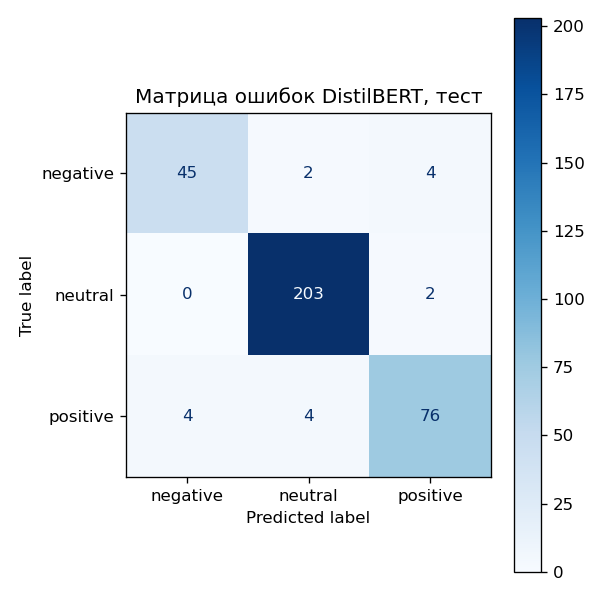
\includegraphics[width=0.62\textwidth]{confusion_matrix.png}
    \caption{Матрица ошибок DistilBERT на тестовой части (строки --- истинные
    классы, столбцы --- предсказанные)}
    \label{fig:cm}
\end{figure}

\begin{table}[H]
    \centering
    \begin{tabular}{lrrr}
        \toprule
        Истина $\backslash$ Предсказание & negative & neutral & positive \\
        \midrule
        negative & 45 & 2 & 4 \\
        neutral  & 0  & 203 & 2 \\
        positive & 4  & 4 & 76 \\
        \bottomrule
    \end{tabular}
    \caption{Матрица ошибок DistilBERT, тестовая часть}
    \label{tab:cm}
\end{table}

Всего 16 ошибок из 340 (4{,}7\,\%). Чаще всего модель путает пару
\texttt{negative}\,$\leftrightarrow$\,\texttt{positive} (по 4 примера в каждую
сторону), а также \texttt{positive}\,$\to$\,\texttt{neutral} (4 примера). Причина в
том, что в финансовых новостях тональность часто выражается не отдельной лексикой, а
смыслом всего предложения, и граница между негативной и позитивной оценкой
оказывается тоньше, чем между нейтральной констатацией и полярным классом. Класс
\texttt{neutral} распознаётся почти идеально (F1~$=0{,}9807$), поскольку он
доминирует в данных.

\textbf{Шаг 3.3. Разбор трёх ошибок} (выбраны наиболее уверенные неверные
предсказания):

\begin{enumerate}
    \item \textit{``Incap Contract Manufacturing Services Private Limited has inked
    agreements with six new customers in India.''} Истина: \texttt{positive},
    предсказание: \texttt{neutral}; вероятности: negative~0{,}0007,
    neutral~0{,}9973, positive~0{,}0020. \textbf{Гипотеза:} по форме это
    нейтральная констатация факта; позитивность проявляется только в финансовом
    смысле (расширение клиентской базы), а выражение ``inked agreements'' не
    входит в позитивные маркеры модели.
    \item \textit{``Mr.~Mikko Saavalainen, head of Comptel's Global Sales concludes:
    ``Gibtelecom provides a perfect illustration of the variety of business,
    technical and regulatory challenges\ldots''} Истина: \texttt{neutral},
    предсказание: \texttt{positive}; вероятности: negative~0{,}0047,
    neutral~0{,}0062, positive~0{,}9891. \textbf{Гипотеза:} слово ``perfect'' ---
    сильный позитивный маркер, хотя здесь ``perfect illustration'' описывает
    сложности, а не даёт оценку компании.
    \item \textit{``In Finland, the city of Forssa has said it will not pay
    compensation to food industry companies HK Ruokatalo and Atria for the lye leak
    into tap water that occurred in March 2008.''} Истина: \texttt{negative},
    предсказание: \texttt{neutral}; вероятности: negative~0{,}0088,
    neutral~0{,}9866, positive~0{,}0047. \textbf{Гипотеза:} негатив (отказ
    компенсировать ущерб от загрязнения воды) выражен через отрицание и юридическую
    формулировку, явно негативной лексики нет, поэтому модель относит текст к
    нейтральному.
\end{enumerate}

\textbf{Шаг 3.4. Эксперимент: качество разметки.} Из зеркала \texttt{ds50}
(согласие не менее 50\,\% аннотаторов) получено 4846 предложений; после исключения
текстов валидации и теста осталось 4165. Из них случайно выбрано 1584 примера ---
столько же, сколько в обучающей части основной постановки, --- и обучена модель с
теми же настройками. Кривые обучения эксперимента приведены в таблице~\ref{tab:exp},
сводный результат --- в таблице~\ref{tab:final}.

\begin{table}[H]
    \centering
    \begin{tabular}{crrrr}
        \toprule
        Эпоха & Train loss & Val loss & Val Accuracy & Val Macro-F1 \\
        \midrule
        1 & 0{,}7711 & 0{,}3500 & 0{,}9353 & 0{,}9054 \\
        2 & 0{,}4224 & 0{,}1976 & 0{,}9647 & 0{,}9462 \\
        3 & 0{,}2705 & 0{,}1411 & 0{,}9618 & \textbf{0{,}9473} \\
        4 & 0{,}1771 & 0{,}1504 & 0{,}9559 & 0{,}9391 \\
        5 & 0{,}1259 & 0{,}1396 & 0{,}9559 & 0{,}9394 \\
        \bottomrule
    \end{tabular}
    \caption{Кривые обучения эксперимента (разметка с согласием $\ge$~50\,\%)}
    \label{tab:exp}
\end{table}

Лучший чекпоинт эксперимента --- эпоха~3 с val Macro-F1~$=0{,}9473$ (здесь ранняя
остановка выбрала модель до последней эпохи, в отличие от основной постановки). На
тестовой части получены Accuracy 0{,}9559 и Macro-F1 0{,}9356 при времени обучения
283{,}1~с.

\begin{table}[H]
    \centering
    \begin{tabular}{lrrr}
        \toprule
        Постановка & Accuracy & Macro-F1 & Время, с \\
        \midrule
        TF-IDF + LogReg (baseline)                        & 0{,}8265 & 0{,}7437 & 0{,}2 \\
        DistilBERT, все аннотаторы согласны (основная)    & 0{,}9529 & 0{,}9321 & 282{,}6 \\
        DistilBERT, согласие $\ge$~50\,\% (эксперимент)   & 0{,}9559 & 0{,}9356 & 283{,}1 \\
        \bottomrule
    \end{tabular}
    \caption{Результат эксперимента шага 3.4 на одной тестовой части}
    \label{tab:final}
\end{table}

\noindent\textbf{Вывод по заданию 3.} Признаков выраженного переобучения нет:
минимум val loss и максимум val Macro-F1 достигаются на последней эпохе, разрыв
val$-$train loss равен $+0{,}1081$, ранняя остановка не сработала. Основные ошибки
(16 из 340) сосредоточены на границе \texttt{negative}/\texttt{positive} и связаны
с неявным, контекстным выражением тональности. Эксперимент с более ``шумной''
разметкой (согласие $\ge$~50\,\%) неожиданно дал даже чуть более высокое качество
(Accuracy 0{,}9559 против 0{,}9529, Macro-F1 0{,}9356 против 0{,}9321 при том же
числе примеров и почти том же времени): расширение пула за счёт предложений с
частичным согласием аннотаторов увеличивает разнообразие обучающих примеров и
улучшает обобщение. Разница невелика (в пределах долей процента) и сопоставима с
шумом на тестовой части из 340 примеров, поэтому трактовать её следует как
отсутствие деградации, а не как гарантированный выигрыш.

\section{Вывод}

В работе решена задача трёхклассовой классификации тональности финансовых новостей
(\texttt{financial\_phrasebank}, разметка \texttt{allagree}) двумя способами.
Классический baseline TF-IDF + логистическая регрессия показал Accuracy 0{,}8265 и
Macro-F1 0{,}7437 при времени обучения 0{,}2~с и слабо распознал редкий класс
\texttt{negative} (Recall~$=0{,}47$). Дообучение DistilBERT за 5 эпох (282{,}6~с)
подняло Accuracy до 0{,}9529 и Macro-F1 до 0{,}9321, то есть качество выросло на
19 процентных пунктов по Macro-F1 ценой примерно в 1400 раз большего времени
обучения. Анализ кривых показал отсутствие выраженного переобучения: минимум
валидационной потери и максимум валидационного Macro-F1 совпадают с последней
эпохой, разрыв val$-$train loss равен $0{,}1081$, ранняя остановка не сработала.
Основные ошибки модели (16 из 340, 4{,}7\,\%) сосредоточены на тонкой границе
между негативной и позитивной оценкой, где тональность выражается контекстом, а не
отдельными словами. Управляемый эксперимент с разметкой, где согласие аннотаторов
не менее 50\,\%, при том же объёме обучающей выборки не ухудшил, а незначительно
улучшил метрики (Accuracy 0{,}9559, Macro-F1 0{,}9356), что говорит об устойчивости
модели к более ``шумной'' разметке.

\end{document}
